\let\negmedspace\undefined
\let\negthickspace\undefined
\documentclass[journal]{IEEEtran}
\usepackage[a5paper, margin=10mm, onecolumn]{geometry}
%\usepackage{lmodern} % Ensure lmodern is loaded for pdflatex
\usepackage{tfrupee} % Include tfrupee package

\setlength{\headheight}{1cm} % Set the height of the header box
\setlength{\headsep}{0mm}     % Set the distance between the header box and the top of the text

\usepackage{gvv-book}
\usepackage{gvv}
\usepackage{cite}
\usepackage{amsmath,amssymb,amsfonts,amsthm}
\usepackage{algorithmic}
\usepackage{graphicx}
\usepackage{textcomp}
\usepackage{xcolor}
\usepackage{txfonts}
\usepackage{listings}
\usepackage{enumitem}
\usepackage{mathtools}
\usepackage{gensymb}
\usepackage{comment}
\usepackage[breaklinks=true]{hyperref}
\usepackage{tkz-euclide} 
\usepackage{listings}
% \usepackage{gvv}                                        
\def\inputGnumericTable{}                                 
\usepackage[latin1]{inputenc}                                
\usepackage{color}                                            
\usepackage{array}                                            
\usepackage{longtable}                                       
\usepackage{calc}                                             
\usepackage{multirow}                                         
\usepackage{hhline}                                           
\usepackage{ifthen}                                           
\usepackage{lscape}
\usepackage{circuitikz}
\tikzstyle{block} = [rectangle, draw, fill=blue!20, 
    text width=4em, text centered, rounded corners, minimum height=3em]
\tikzstyle{sum} = [draw, fill=blue!10, circle, minimum size=1cm, node distance=1.5cm]
\tikzstyle{input} = [coordinate]
\tikzstyle{output} = [coordinate]



\graphicspath{{figs/}}
\renewcommand{\theequation}{2.8.5.\arabic{equation}}
\renewcommand{\thefigure}{2.8.5.\arabic{figure}}

\bibliographystyle{IEEEtran}
\vspace{1.5em}

\title{2.8.5}
\author{E Achyuta Siddartha - ee25btech11024}

\begin{document}
\maketitle

\noindent
\textbf{Problem Statement} \\
A line makes angles $\alpha, \beta, \gamma$ and $\delta$ with the diagonals of a cube, prove that
\begin{align}
\cos^2\alpha + \cos^2\beta + \cos^2\gamma + \cos^2\delta = \frac{4}{3}
\end{align}

\vspace{1.5em}

\noindent
\textbf{Solution:}\\

\begin{center}
    \begin{tabular}{|c|c|p{5cm}|}
    \hline
    \textbf{Symbol} & \textbf{Value} & \textbf{Description}  \\
    \hline
    \textbf{$\vec{D}_1, \vec{D}_2, \vec{D}_3, \vec{D}_4$} & $\myvec{1\\1\\1}, \myvec{-1\\1\\1}, \dots$ & Column vectors for the four cube diagonals \\
    \hline
    \textbf{$\vec{L}$} & $\myvec{l \\ m \\ n}$ & Line's unit direction vector, where $\vec{L}^\top\vec{L} = 1$ \\
    \hline
    \end{tabular}
\end{center}
\noindent

\noindent
For angle $\theta_i$ between the line $\vec{L}$ and a diagonal $\vec{D}_i$,
\begin{align}
    \cos\theta_i = \frac{\vec{L}^\top \vec{D}_i}{\|\vec{L}\| \|\vec{D}_i\|} = \frac{\vec{L}^\top \vec{D}_i}{\sqrt{3}}
    \label{eq:2.8.5.1}
\end{align}
Since $\vec{L}^\top \vec{D}_i$ is a scalar, it equals its own transpose, so 
\begin{align}
(\vec{L}^\top \vec{D}_i)^2 = (\vec{L}^\top \vec{D}_i)(\vec{D}_i^\top \vec{L}).  
\label{eq:2.8.5.2}
\end{align}
using \eqref{eq:2.8.5.1} and \eqref{eq:2.8.5.2} to find S i.e sum of squares,
\begin{align} 
    S = \sum_{i=1}^{4} \cos^2\theta_i = \sum_{i=1}^{4} \frac{(\vec{L}^\top \vec{D}_i)(\vec{D}_i^\top \vec{L})}{3} = \frac{1}{3} \vec{L}^\top \left( \sum_{i=1}^{4} \vec{D}_i \vec{D}_i^\top \right) \vec{L}
    \label{eq:quad.form}
\end{align}
The expression $\vec{D}_i \vec{D}_i^\top$ is the \textbf{outer product} of the vector with itself. Let's calculate the matrix $M = \sum_{i=1}^{4} \vec{D}_i \vec{D}_i^\top$.
\begin{align}
    \vec{D}_1\vec{D}_1^\top &= \myvec{1\\1\\1}\myvec{1\\1\\1}^\top = \myvec{1&1&1\\1&1&1\\1&1&1}\quad
    \vec{D}_2\vec{D}_2^\top = \myvec{-1\\1\\1}\myvec{-1\\1\\1}^\top = \myvec{1&-1&-1\\-1&1&1\\-1&1&1} \nonumber \\
    \vec{D}_3\vec{D}_3^\top &= \myvec{1\\-1\\1}\myvec{1\\-1\\1}^\top = \myvec{1&-1&1\\-1&1&-1\\1&-1&1} \quad
    \vec{D}_4\vec{D}_4^\top = \myvec{1\\1\\-1}\myvec{1\\1\\-1}^\top = \myvec{1&1&-1\\1&1&-1\\-1&-1&1} \nonumber
\end{align}
By adding these four matrices we get,
\begin{align}
    M = \sum_{i=1}^{4} \vec{D}_i \vec{D}_i^\top = \myvec{4&0&0\\0&4&0\\0&0&4}= 4I
    \label{eq:outer.product.sum}
\end{align}
Substituting\eqref{eq:outer.product.sum} in \eqref{eq:quad.form} we get,
\begin{align}
    S = \frac{1}{3} \vec{L}^\top (4I) \vec{L} = \frac{4}{3} \vec{L}^\top I \vec{L} = \frac{4}{3} \vec{L}^\top \vec{L}
\end{align}
Since $\vec{L}$ is a unit vector, $\vec{L}^\top \vec{L} = \|\vec{L}\|^2 = 1$.
\begin{align}
    S = \frac{4}{3}(1) = \frac{4}{3}
\end{align}
Thus, it is proven that 
\begin{align*}
\cos^2\alpha + \cos^2\beta + \cos^2\gamma + \cos^2\delta = \frac{4}{3}.
\end{align*}

See Figure~\ref{fig:3DVectors}.

\begin{figure}[h!]
    \centering
    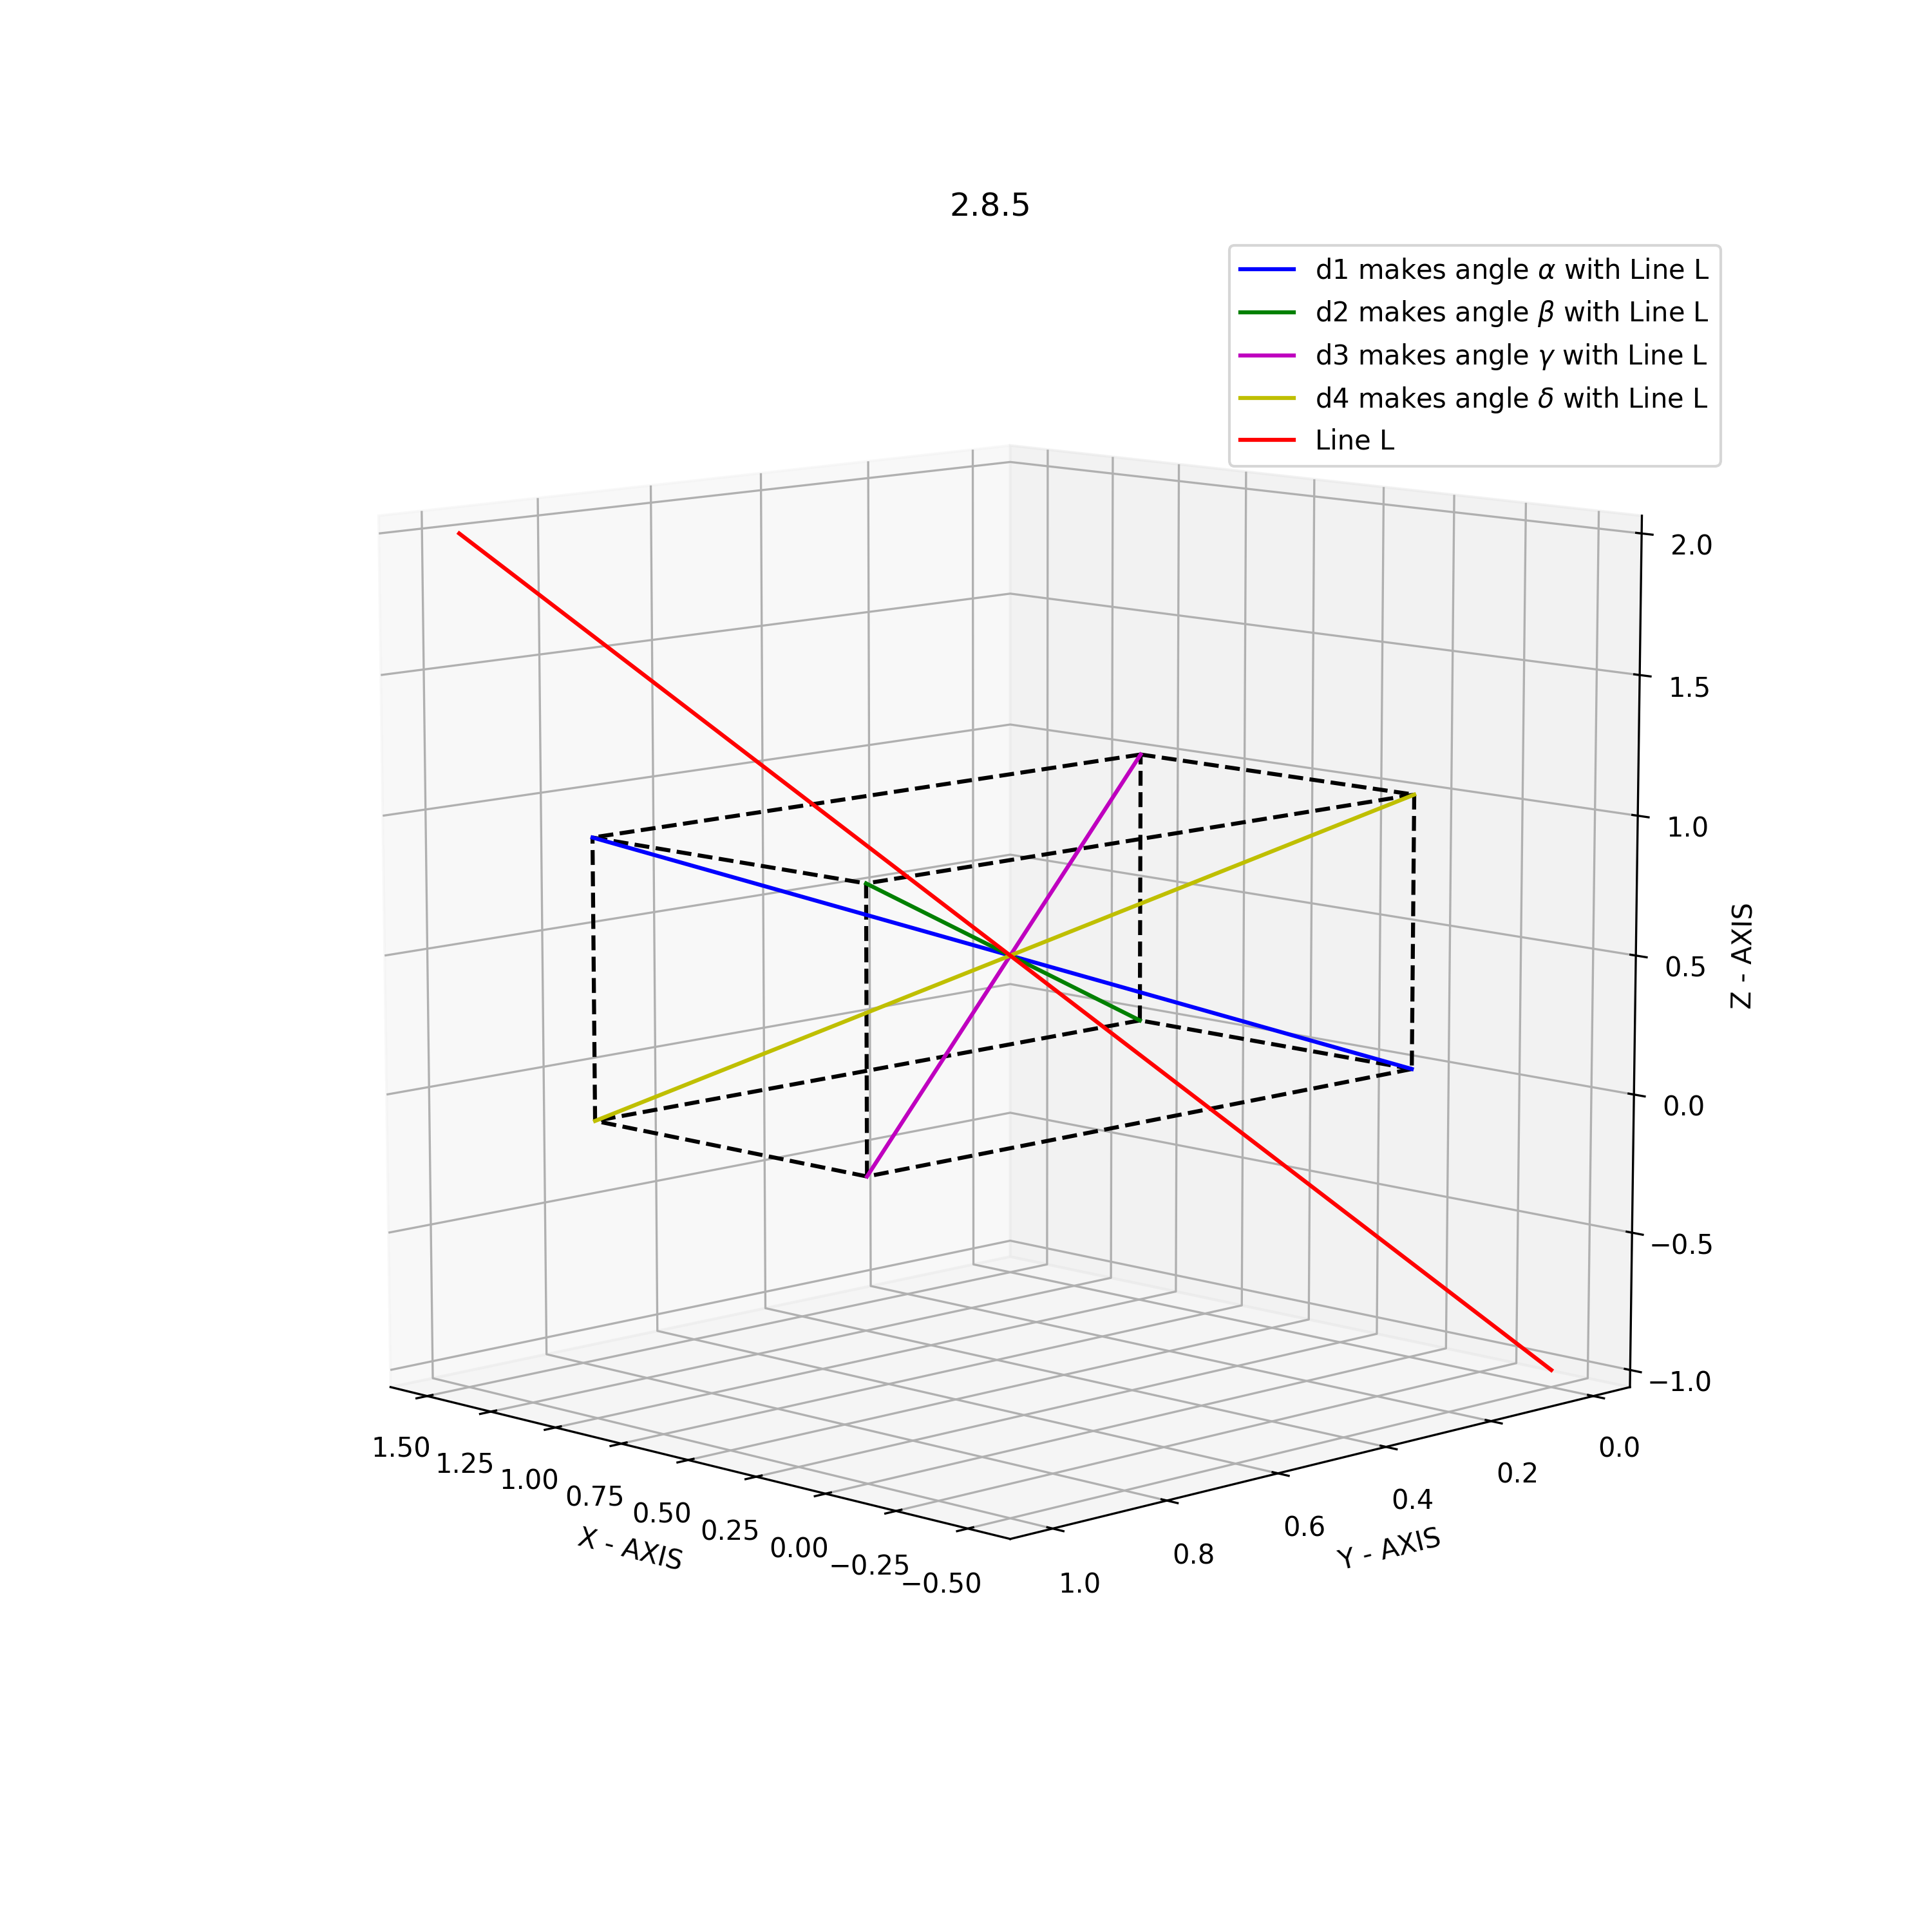
\includegraphics[width=1.0\linewidth]{figs/fig4.png}
    \caption{}
    \label{fig:3DVectors}
\end{figure}



\end{document}

